\section{Methodology}
To measure the SIDIS events, one needs a source of high energy electrons, a detector system capable of measuring the final state electron and hadron, and a computing cluster to perform data processing and analysis.  All of these facilities are provided by Jefferson National Lab, which houses an electron accelerator known as CEBAF, the CLAS spectrometer for detection, and a moderate sized computing cluster for data processing.  In addition to these facilities, a set of analysis techniques and procedures is needed to complete this thesis study.  This section details the methodology used to complete this thesis, comprised of the experimental facility and procedure as well as the data analysis procedure.

\subsection{Experimental Facility}
Jefferson Lab is home to the Continuous Electron Beam Accelerator Facility (CEBAF).  It houses 4 state of the art experimental end-stations for fixed target collisions of electrons or photons on various targets.  CEBAF begins with a 45-MeV electron injector.  The accelerator consists of two linear accelerators (north and south LINACs) and a set of 4 recirculating arcs at both ends of the race track shaped facility.  Electrons are passed through the LINACs up to 4 times, gaining 1.14 GeV each pass.  CEBAF was designed to generate up to 6 GeV electron beams, and has now been upgraded to provide 12 GeV electrons. Electrons are delivered to the halls in bunches of approximately 1 million at 2 ns intervals.

\subsubsection{CLAS in Hall-B}
Hall-B contains the CEBAF Large Acceptance Spectrometer (CLAS) a large spherical detector capable of measuring final state particles with a large range of momentum and angles.  CLAS has the ability to measure exclusive reactions, reconstructing the 4-vectors of all final state particles involved in the reaction.  In cases where one particle is not detected, CLAS also has the resolution to resolve them from missing mass spectra.  This is achieved by combining several different types of detectors into one package, which will be described below.  The CLAS detector has now been dismantled and replaced with CLAS12, but the following sections describe CLAS as it was at the time of data taking for the E1-F experiment used in this thesis.  The major components of CLAS \cite{clas} are designed to identify different types of particles at different ranges of momenta, they are:

\begin{figure}
  \centering
  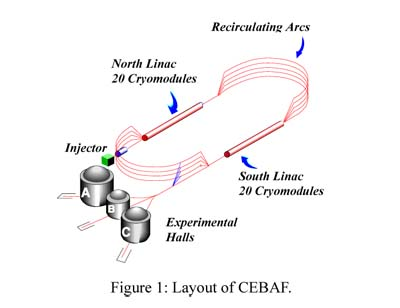
\includegraphics[width=10cm]{image/cebaf.jpg}
  \caption{ Diagram showing how CEBAF is constructed.  }
  \label{fig:jlab}
\end{figure}

\easyFigure{image/no-image.jpg}{This image will be added later.}

\begin{itemize}
\item Large Torus Magnet - The torus is the central bending magnet which creates a toroidal magnetic field and dictates the design of almost all other detectors.  The torus consists of 6 superconducting coils, (operated at up to 3860 Amperes) which seperate the forward detector systems into 6 distict sectors.  The torus magnet can be used to bend charged particles toward or away from the beamline, and creates the field necessary to determine charge and momentum of particles incident on the CLAS detectors.  
\item Drift Chamber systems - A total of 18 drift chambers are used, 3 radially seperated chambers per sector which are refered to as ``Regions 1-3''.  The primary role of the drift chambers is to provide charge identification and momentum by measuring the bend of the particle as it passes through the known magnetic field.    
\item Cherenkov Light Counters - CLAS is equipped with 6 Cherenkov light counters, filled with $C_{4} F_{10}$.  The Cherenkov Counters (CC) serve two purposes.  The CC serves as a trigger for electrons, and also separates electrons from negative pi-mesons $\pi^{-}$ below 2.5 GeV/c.
\item Scintillating Time Of Flight Panels - Scintillating time of flight (TOF) counters offer coverage from $8^{\circ} - 142^{\circ}$ in the polar angle.  The primary function of the TOF system is to provide timing information to differentiate between particles of different mass based on their time of flight and momentum.  
\item Electromagnetic Calorimeter - The last layer of detection is the electromagnetic calorimeter (EC), which consists of alternating layers of lead and scintilation material.  Electrons and photons can be detected from the shower they leave behind as they pass through the EC.  The EC was designed to have a layered structure, so as to provide hit position information as the particle passes through each layer.  The EC is vital in reconstructing neutrals which strongly decay into photons (such as $\pi^0, \eta$). See figure \ref{fig:ec_clas}.  
\end{itemize}

\begin{figure}
  \centering
  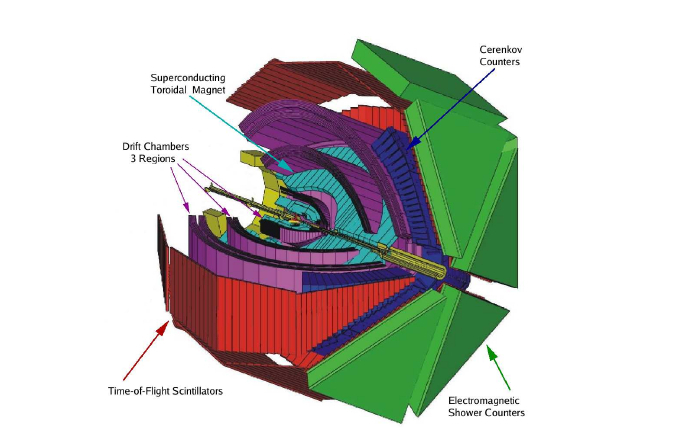
\includegraphics[width=10cm]{image/clas.png}
  \caption{ Computer Rendering of CLAS with detector subsystems labeled.}
  \label{fig:clas}
\end{figure}

\begin{figure}
  \centering
  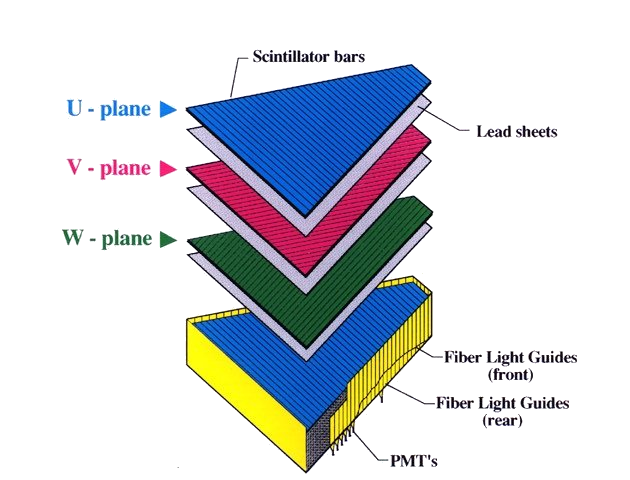
\includegraphics[width=10cm]{image/ec.png}
  \caption{The CLAS electromagnetic calorimeter}
  \label{fig:ec_clas}
\end{figure}

\subsection{Data Analysis}
Analysis of the data taken by the CLAS detector is a process which starts with reconstruction of the raw data (electrical signals recorded by ADC and TDC components).  The reconstruction algorythm builds particle tracks by finding the best possible track through a set of detector hits.  The result is a set of files with charge, momentum, timing, and preliminary particle identification information for each event.  The reconstruction package is the critical first step to a data analysis, and the interested reader can find more details in \cite{reconstruction-doc}.  The first task for most analysists is the identification of electrons.

\subsubsection{Electron Identification}
All negative tracks start out as electron candidates, they are accepted if they pass a series of identification cuts. The ratio $E_{Dep}/p$ is calculated for each track, and because electrons have a very constant ratio as a function of momentum, we can use this ratio to separate them from minimally ionizing particles ($\pi^{-}$ being the most dominant background).  Exploiting this same logic, a cut is placed on the minimum energy deposited in the electromagnetic calorimeter inner layers.Tracks that pass these cuts are next subjected to a variety of geometric cuts to ensure that they pass through regions of the detectors that are well understood.  Tracks passing too close to the edges of the electromagnetic calorimeters can shower outside of the detector leading to incorrect reconstruction of energy for that particle.  Finally, cuts are applied to the Cherenkov counter signal.  Often, charged pions do not have enough momentum $p \leq 2.4 GeV/c$ to participate in the Cherenkov Effect and no signal is preset in the Cherekov Counter.  By requiring a signal in the Cherenkov we remove these events.  We then apply matching cuts to the detection angle of the track in the Cherenkov Counter and the number of the PMT which detected the track (these should be 1-to-1 correlated).  These proceedures are summarized in detail in the following note \cite{electron-note}.

\begin{figure}
  \centering
  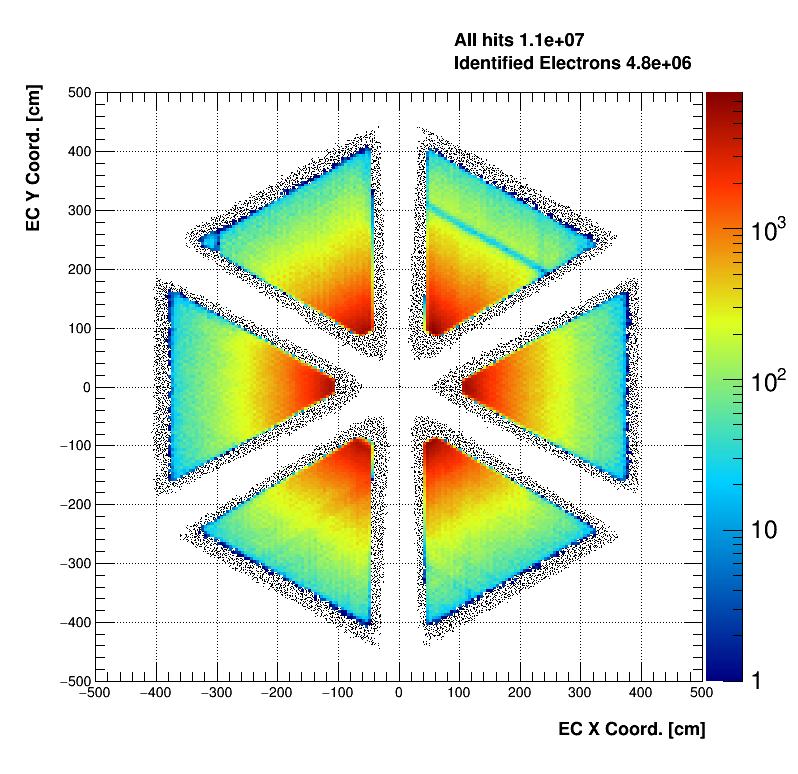
\includegraphics[width=9cm]{image/ECFiducial.png}
  \caption{Electromagnetic (EC) calorimeter negative track hits.  Shown in black, negatives tracks rejected in electron identification.  Hits close to the borders of the EC incompletely shower and can reconstruct with incorrect energy.}
  \label{fig:ecfid}
\end{figure}

\subsubsection{Kaon Identification}
If an event contains a good electron, the rest of the event is processed.  Kaons are identified based on time of flight information.  In this analysis, we use a maximum likelihood ratio technique to classify all positive tracks as either pions, kaons, or protons.  Finally, we control the track quality by requiring a significance level of $\alpha = 0.05$.  These procedures are described in detail in the following note \cite{kaon-note}.

\subsection{EVA Framework}
The Evaluation and VAlidation (EVA) project is a project on-going at the University of Connecticut and Jefferson Lab.  The goal of EVA is to build a tool that can be used to extract TMD functions from data taken during CLAS12 operation, as well as global data from other collaborations/experiments.  As a form of validation, EVA will have the ability to generate physics events based on some physics model and a set of parameters.  These events can be fed into the particle swimming detector simulation for CLAS12, and the results can be analyzed.  The EVA framework can then extract from the simulated data the parameters in the chosen model.  These parameters can be compared with the starting point in the EVA chain. \\

For this work, we will use EVA to extract parameters of the Boer-Mulders TMD function from our measurement of the SIDIS cross section.  The parametrization used will be described fully in the dissertation work.
